\sezione{Esercizio di Dimensionamento}
Si consideri il sistema in esame formato da motore, riduttore, vite, madrevite, carico e con una legge di moto come in figura.\label{EsercizioDimRid}

\begin{figure}[h]
    \centering
    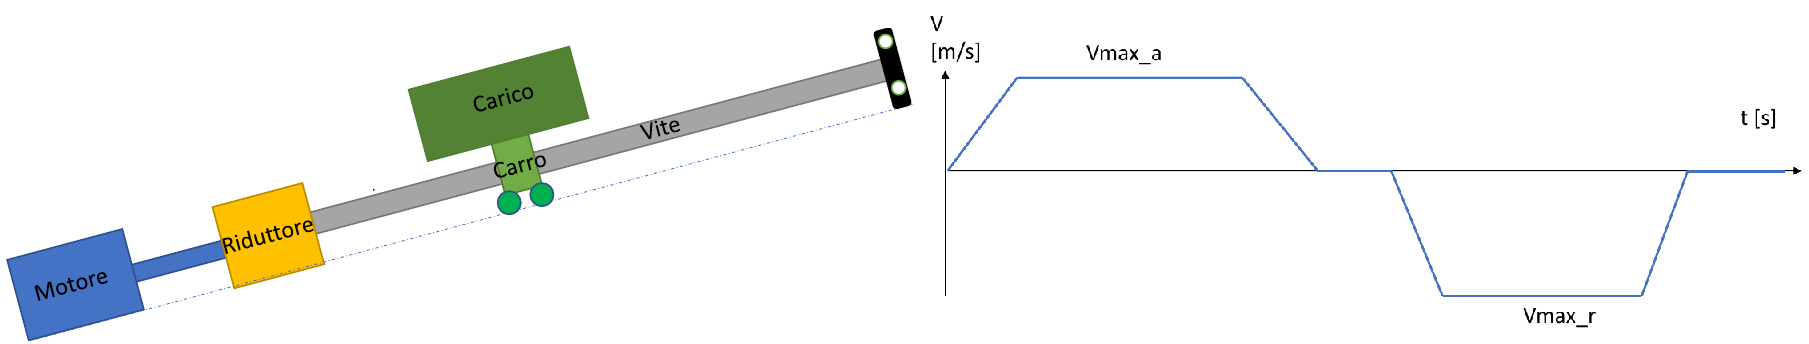
\includegraphics[width=0.8\textwidth]{Immagini/esercizio1_dim_rid_vite.png}
    \caption{Esercizio 1 dimensionamento: schema e legge oraria}
\end{figure}

\paragrafo{Utilizzo di F:}
Al posto di considerare le forze come singole, considero di unire tutti le forze come unico contributo. Questo permette di mantenere una buona coerenza dei segni.

\paragrafo{Rendimento:}
Viene utilizzato il rendimento generalizzato, dove \(\eta_v^d=0.9\), quindi \(\eta_v^r \simeq 2-\frac{1}{\eta_v^d}=\frac{1}{1.125}\), ossia 
\[
\begin{cases}
    \eta_v^d = 0.9 \text{ \ se \ } -\dot{x}F_a < 0 \\
    \frac{1}{\eta_v^r} = 1.125  \text{ \ se \ } -\dot{x}F_a \geqslant 0
\end{cases}
\]

\sottosezione{Step di risoluzione}
\begin{enumerate}[label=(\roman*)]
    \item Convenzioni di segno (intanto raggruppando le forze applicate su uno stesso punto)
    \item Modello (cinematico, dinamico)
    \item Manipolazione algebrica del modello per evidenziare $T_2$ ed eventualmente le forze che vanno a determinare il tipo di moto (diretto vs retrogrado)
    \item Analisi di ogni fase
    \item Valutazione del duty cycle
    \item Definizione $T_2$, scelta taglia
    \item Calcolo limitazioni alla scelta di $\tau_r$
    \item Scelta di $\tau_r$
\end{enumerate}

\sottosezione{Tabella}
Per aiutarsi nella esecuzione dei passaggi è consigliato l'utilizzo di una tabella in cui siano distinte le varie tipologie operative divise per le rispettive durate di modo da schematizzare l'esercitazione.

\begin{table}[h]
\centering
    \begin{tabular}{c|c|c|c|c|c|c|c|c|c}
    \hline
    $\Delta t$ $[s]$ & $0.4$ & $1.2$ & $0.4$ & $0.4$ & $0.3$ & $0.9$ & $0.3$ & $0.6$ & Max \\ \hline
    $\dot x$ $[m/s]$ & >0 & \(0.75\) & >0 & 0 & <0 & -1 & <0 & 0 & 1 \\ \cline{1-1}
    $\Ddot x$ $[m/s^2]$ & 1.875 & 0 & -1.875 & 0 & -3.333 & 0 & 3.333 & 0 &  \\ \cline{1-1}
    $M$ $[Kg]$ & 670 & 670 & 670 & 670 & 70 & 70 & 70 & 70 &  \\ \cline{1-1}
    \hline
    $M \Ddot x$ $[N]$ & \(1256.3^R\) & 0 & \(-1256.3^M\) & 0 & \(-233.3^R\) & 0 & \(233.3^M\) & 0 &  \\ \cline{1-1}
    $F_{p,\parallel}$ $[N]$ & 2774.9 & 2774.9 & 2774.9 & 2774.9 & 289.9 & 289.9 & 289.9 & 289.9 &  \\ \cline{1-1}
    $F_{cou}$ $[N]$ & 892.6 & 892.6 & 892.6 & \(-892.6^*\) & -93.3 & -93.3 & -93.3 & -93.3 &  \\ \cline{1-1}
    $\Delta F_{cou}^s$ $[N]$ & (297.5) & - & - & -297.5 & (-31.1) & - & - & -31.1 &  \\ \cline{1-1}
    \hline
    $F_{A,medi}$ $[N]$ & 4929.8 & 3667.5 & 2411.3 & 1587.7 & -36.7 & 196.7 & 430 & 165.6 &  \\ \cline{1-1}
    $F_{A,pk}$ $[N]$ & 5221.3 &  &  &  & -67.8 &  &  &  &  \\ \cline{1-1}
    Flusso $W$ & D & D & D & "R" & D & R & R & "R" &  \\ \cline{1-1}
    \hline
    $\VelAng_v$ $[rpm]$ &  & 750 &  & 0 &  & -1000 &  & 0 &  \\ \cline{1-1}
    $\AccAng_v$ $[rd/s]$ & 196.3 & 0 & -196.3 & 0 & -34.9 & 0 & 34.9 & 0 &  \\ \cline{1-1}
    \hline
    $J_v\AccAng_v$ $[Nm]$  & 0.57 & 0 & -0.57 & 0 & -1.01 & 0 & 1.01 & 0 &  \\ \cline{1-1}
    $T_2$ $[Nm]$ & 52.8 & 38.9 & 25 & 17 & -1.4 & 2.1 & 5.6 & 1.8 &  \\ \cline{1-1}
    $T_{2,pk}$ $[Nm]$ & (56) &  &  &  &  &  &  &  & 56 \\ \cline{1-1}
    \hline
    \end{tabular}
    \caption{Tabella riassuntiva per i calcoli effettuati}
\end{table}

\paragrafo{Incremento di Attrito:}
Con $\Delta F_{Cou}$ si intende l'incremento di attrito legato alla differenza tra attrito statico e dinamico; nota bene che $\Delta F_{Cou} + F_{Cou} \leqslant F_{motrice}$: l'incremento potrà al massimo far sì che l'oggetto rimanga fermo, non può metterlo in moto.

\paragrafo{Attrito di Primo Distacco:}
L'attrito statico è di primo distacco interviene quando si passa da arresto a moto, tuttavia il tempo di applicazione dell'attrito è trascurabile rispetto il ciclo di lavoro, perciò può influenzare il valore di picco di forza\footnote{Questo non andrà a influenzare la scelta del motore perché i motori brushless tendono ad avere coppie di spunto alte a sufficienza per garantire il primo distacco.}, ma non la media. Questi casi conviene segnarli in tabella mettendo il valore dentro parentesi tonde.

\paragrafo{Verifica segni:}
Per verificare di aver utilizzato tutte le convezioni corrette conviene partire dai segni dell'inerzia, valutare in base alla legge oraria quale sia il segno dell'inerzia resistente e quale dell'inerzia motrice, e infine estendere quanto ricavato alle altre forze, quindi verificare che le forze resistenti e motrici siano concordi coi segni delle rispettive inerzie.
Nell'esempio occorrerà valutare il segno dell'inerzia resistente e motrice nelle condizioni di salita e discesa.

\sottosezione{Valutazioni su riduttore}
I parametri da ricavare per il riduttore sono:
\begin{itemize}
    \item Duty cycle \(\delta = 78\% \)
    \item Limite di coppia applicabile in modo continuativo \(T_{2,B} = T_2^\text{max,richiesta} f_s \cdot 1.2 = 74 Nm \)
    \item Coppia nominale richiesta \(T_{2,N} = \sqrt[3]{\frac{\sum^3_{i=1}\abs{T_{2,i}^3\Delta t_i \VelAng_{v,i}}}{\sum^3_{i=1} \abs{\Delta t_i \VelAng_{v,i}} }} \cdot 1.2 = 39 Nm\), dove nelle fasi ad accelerazione costante viene considerata la velocità media nel tratto
\end{itemize}
Con questi valori posso andare a catalogo e scegliere una taglia; risulta HPS75 (o superiore), che ha \(n_{1,max} = 6000 rpm\) e \(n_{1,N} = 2500\div 3000\).

\paragrafo{Rapporto di trasmissione minimo per velocità massima:}
Ottenuta la velocità è possibile ricavare il valore minimo di rapporto di trasmissione da utilizzare per garantire la velocità massima: \(\tau_{R,min} = \frac{\VelAng_{R,max}}{n_{1,max}} 0.8 = \frac{1}{4.8}\), perciò le scelte disponibili sono limitate a \(\tau=\frac{1}{4}\).

\paragrafo{Rapporto di trasmissione minimo per velocità media:}
Nota la velocità media richiesta al carico posso ottenere la velocità media richiesta in uscita dal riduttore \(\VelAng_{v,media} = \frac{\dot{x}_{media}\frac{60}{2\pi}}{\tau_v} = 533 rpm\), da cui ottengo un rapporto di trasmissione minimo di \(\tau_{R,min} = \frac{\VelAng_{v,media}}{\dot{x}_{media}} 0.8 = 3.75 < 4\), ossia il limite è eccessivamente stringente.

\paragrafo{Rivalutazione coefficiente di sicurezza:}
Facendo l'esercizio ci si accorge che utilizzando un coefficiente di sicurezza del $20\%$ non si trova un riduttore tra quelli a disposizione perché la velocità media richiesta è troppo elevata. L'unica opzione\footnote{Vedi quanto detto a pagina \pageref{rivalutazione_coeff_sic}} è modificare il coefficiente di sicurezza.
Facendo una valutazione di potenze media richiesta: \(W_{media}^{richiesta}=T_{2,media}^R \VelAng^R_{media}=32.7\cdot 533 = 17430 Nmrpm\) contro la potenza media nominale del riduttore con rapporto di riduzione di \(\tau=\frac{1}{4}\), \(W_{N} = T_{2,N} n_{1,N}\tau_R = 60 \frac{2500}{4} = 37500 Nm rpm\).
Si osserva come in questo caso la $T_{2,media}$ è circa la metà di quella nominale, perciò termicamente il rischio è minimo, quindi è possibile abbassare il coefficiente di sicurezza relativo alla velocità media e scegliere \(\tau = \frac{1}{4}\).